\chapterold{Puntatori}
\myindex{\CLanguageElements!\Pointers}
\label{label_pointers}

I puntatori sono spesso usati per restituire valori dalle funzioni (come nel caso di \scanf ~(\myref{label_scanf})).
Ad esempio, quando una funzione deve restituire due valori.

\sectionold{Global variables example}

\lstinputlisting{patterns/061_pointers/global.c}

Viene compilato in:

\lstinputlisting[caption=\Optimizing MSVC 2010 (/Ob0)]{patterns/061_pointers/global.asm}

\myindex{\olly}
\clearpage
Esaminiamolo con \olly:

\begin{figure}[H]
\centering
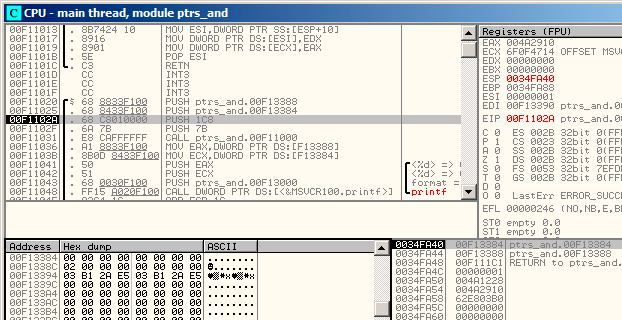
\includegraphics[scale=\FigScale]{patterns/061_pointers/olly_global1.png}
\caption{\olly: 
global variables addresses are passed to \ttfone}
\label{fig:pointers_olly_global_1}
\end{figure}

Prima di tutto, gli indirizzi delle variabili globali vengono passati a \ttfone.
Possiamo cliccare su \q{Follow in dump} sull'elemento dello stack e vedere lo spazio nel data segment allocato per le due variabili.

\clearpage
Queste variabili sono azzerate, poiche' i dati non inizializzati (dal segmento \ac{BSS}) sono azzerati prima dell'inizio dell'esecuzione: [\CNineNineStd 6.7.8p10].

Risiedono nel data segment, e possiamo verificarlo premendo Alt-M ed esaminando la mappa della memoria:

\begin{figure}[H]
\centering
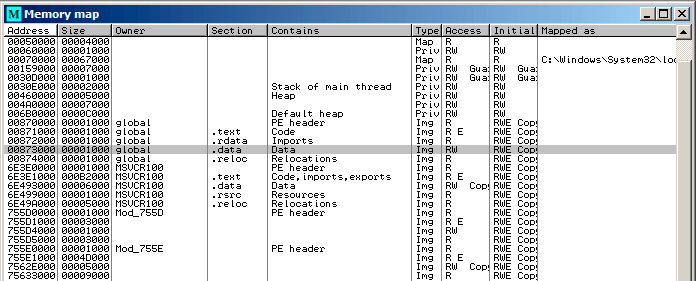
\includegraphics[scale=\FigScale]{patterns/061_pointers/olly_global5.png}
\caption{\olly: memory map}
\label{fig:pointers_olly_global_5}
\end{figure}

\clearpage
Eseguiamo (F7) fino all'inizio di \ttfone: 

\begin{figure}[H]
\centering
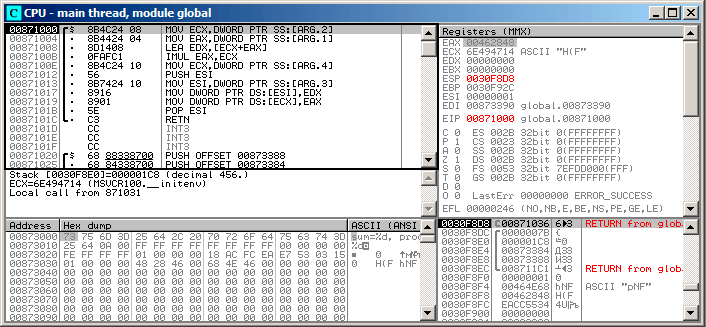
\includegraphics[scale=\FigScale]{patterns/061_pointers/olly_global2.png}
\caption{\olly: \ttfone starts}
\label{fig:pointers_olly_global_2}
\end{figure}

Nello stack sono visibili due avlori, 456 (\TT{0x1C8}) e
123 (\TT{0x7B}), oltre agli indirizzi delle due variabili globali.

\clearpage

Eseguiamo fino alla fine di \ttfone.
Nella finestra in basso a sinistra vediamo come i risultati dei calcoli appaiono nelle viariabili globali:

\begin{figure}[H]
\centering
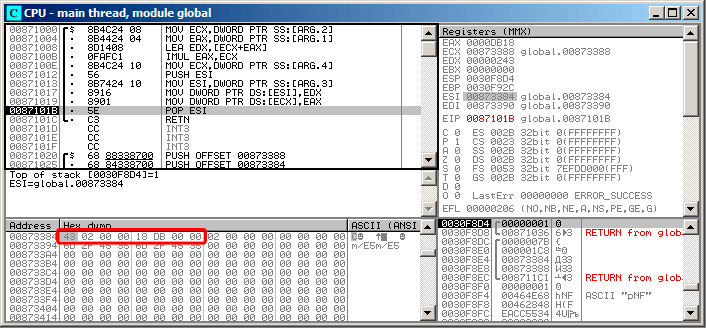
\includegraphics[scale=\FigScale]{patterns/061_pointers/olly_global3.png}
\caption{\olly: \ttfone execution completed}
\label{fig:pointers_olly_global_3}
\end{figure}

\clearpage

Adesso i valori delle variabili globali sono caricati nei registri, pronti per essere passati a \printf (tramite lo stack):

\begin{figure}[H]
\centering
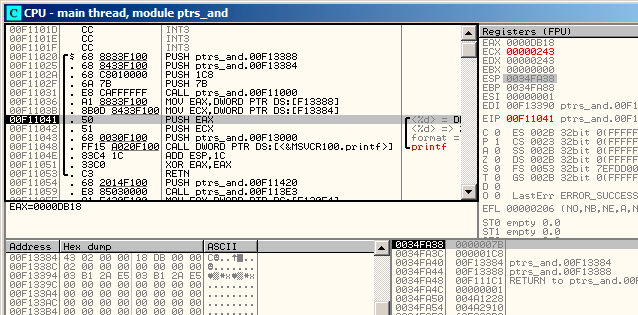
\includegraphics[scale=\FigScale]{patterns/061_pointers/olly_global4.png}
\caption{\olly: 
global variables' addresses are passed into \printf}
\label{fig:pointers_olly_global_4}
\end{figure}

\sectionold{Local variables example}

Aggiustiamo leggermente l'esempio:

\lstinputlisting[caption=adesso le variabili \TT{sum} e \TT{product} sono locali]{patterns/061_pointers/local_EN.c}

Il codice di \ttfone restera' invariato.
Solo \main cambiera' in:

\lstinputlisting[caption=\Optimizing MSVC 2010 (/Ob0)]{patterns/061_pointers/local.asm}

\clearpage
Esaminiamo nuovamente con \olly.
Gli indirizzi delle variabili locali nello stack sono \TT{0x2EF854} e \TT{0x2EF858}.
Vediamo come questi vengono messi nello stack: 

\begin{figure}[H]
\centering
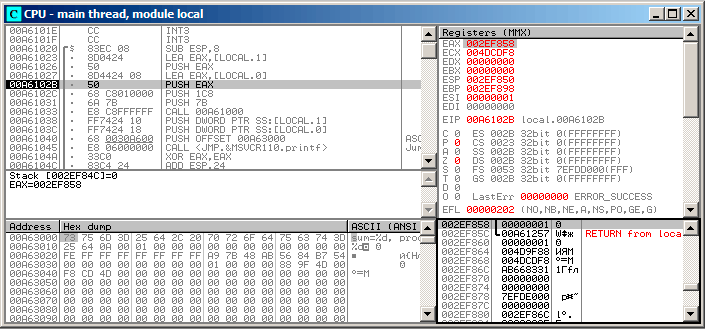
\includegraphics[scale=\FigScale]{patterns/061_pointers/olly_stk1.png}
\caption{\olly: local variables' addresses are
pushed into the stack}
\label{fig:pointers_olly_stk_1}
\end{figure}

\clearpage
Inizia \ttfone.
A questo punto nello stack c'e' solo random garbage a \TT{0x2EF854} e \TT{0x2EF858} :

\begin{figure}[H]
\centering
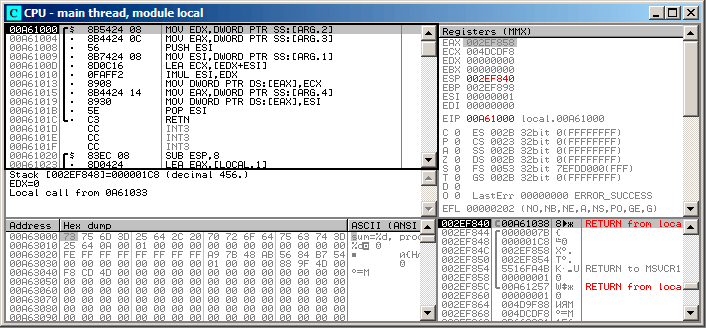
\includegraphics[scale=\FigScale]{patterns/061_pointers/olly_stk2.png}
\caption{\olly: \ttfone starting}
\label{fig:pointers_olly_stk_2}
\end{figure}

\clearpage
\ttfone finisce:

\begin{figure}[H]
\centering
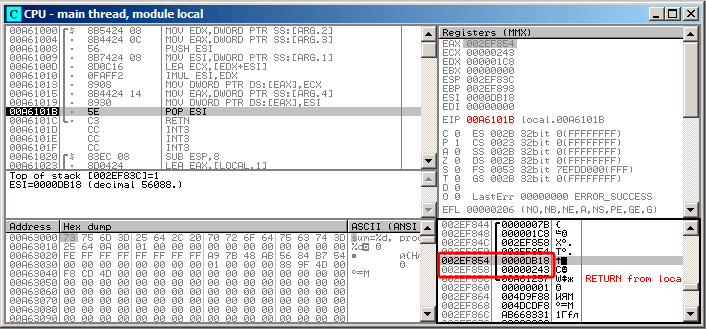
\includegraphics[scale=\FigScale]{patterns/061_pointers/olly_stk3.png}
\caption{\olly: \ttfone completes execution}
\label{fig:pointers_olly_stk_3}
\end{figure}

Adesso agli indirizzi \TT{0x2EF854} e \TT{0x2EF858} vediamo \TT{0xDB18} e \TT{0x243}.
Questi valori sono il risultato di \ttfone.

\sectionold{\Conclusione{}}
 
\ttfone puo' restituire puntatori ad un qualunque posto in memoria, a prescindere da dove si trovi.
In definitiva e' questa l'utilita' dei puntatori.

A proposito, le \IT{references} di \Cpp funzionano esattamente allo stesso modo.
Maggiori dettagli qui: (\myref{cpp_references}).
